\chapter{Rätselseite}

\textbf{Mini-Sudoku}: Trage in jede Zeile und Spalte
  die Ziffern 1, 2, 3,~4 so ein, dass A~waagrecht, A~senkrecht,
  B~senkrecht und F~senkrecht Primzahlen sind!\\[0.2cm]
\begin{tabular}{ |p{0.8cm}|p{0.8cm}|p{0.8cm}|p{0.8cm}| }
\hline
  a & b & c & d \\[0.8cm]
\hline
  e &   &   &   \\[0.8cm]
\hline
  f &   &   &   \\[0.8cm]
\hline
  g &   &   &   \\[0.8cm]
\hline
\end{tabular}

\medskip
\textbf{Löse folgende Gleichung:}

\[\frac{\textrm{EVE}}{\textrm{D\,I\,D}} = \textrm{0,TALKTALKTALK}\dots\]

Jeder Buchstabe steht für eine andere Ziffer.

\textbf{Visitenkarten:} Welchen Beruf haben diese Personen?\\

\centerline{Hanne Rubbich \textendash{} Ilztal\\[0.2cm]}
\centerline{Richie Hersvogt \textendash{} Zell\\[0.2cm]}
\centerline{Meike Schmettelin \textendash{} Berlin\\[0.2cm]}

\medskip
\textbf{Minesweeper:} Kennst du.  Jedes Level ist eindeutig lösbar.\\[0.2cm]
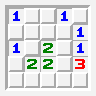
\includegraphics[width=0.45\linewidth]{minepuzzle_gen02tr.png}
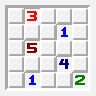
\includegraphics[width=0.45\linewidth]{minepuzzle_gen14tr.png}

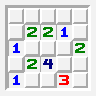
\includegraphics[width=0.45\linewidth]{minepuzzle_gen18tr.png}
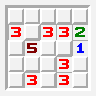
\includegraphics[width=0.45\linewidth]{minepuzzle_gen21tr.png}

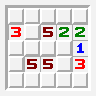
\includegraphics[width=0.45\linewidth]{minepuzzle_gen29tr.png}
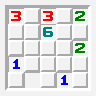
\includegraphics[width=0.45\linewidth]{minepuzzle_gen19tr.png}

\bigskip
\textbf{Kreuzzahlenrätsel:} Jede Summe, und jeder Summand innerhalb der Summe, darf nur einmal auftreten.

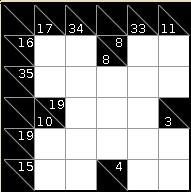
\includegraphics[width=0.9\linewidth]{2011-10-02-134837_191x192_scrot.png}

\end{multicols}

